% 2 Oort-Lindbladモデルと観測方程式 (仮)
% 2.1 速度分散の無い系の太陽運動と銀河速度場 ← 宮本ノートや藤田修論を参考に書く
% 2.1.1 Oort-Lindbladモデル ← A, B, C, Kの導出と物理的意味
% 2.1.2 観測方程式 ← 従来のもの

% 2.2 速度分散を考慮した場合への拡張 ← Olling & Dehnenを参考に書く
% 2.2.1 従来のOort-Lindbladモデルの問題点 ← ここにYu & Liu の年齢速度分散関係の図も載せるとよい。
% 2.2.2 asymmetric drift ← 導出&物理的解釈を書く
% 2.2.3 asymmetric driftを考慮した観測方程式


\chapter{Oort-Lindbladモデルと観測方程式 \label{chap2}}
この章では、本研究で用いているOort-Lindbladモデルと、実際に観測データにこのモデルを適用する観測方程式の説明をする。まず、速度分散の無い系でのOort-Lindbladモデルと観測方程式について説明する。その後、従来のOort-Lindbladモデルの問題点と、速度分散を考慮した場合に考えるべき効果に加えて、そのような場合に拡張した観測方程式の説明をする。
\section{速度分散の無い系の太陽運動と銀河速度場} % 宮本ノートや藤田修論を参考に書く
この節では、速度分散の無い系での太陽運動とOort-Lindbladモデル、銀河系の速度場について説明する。太陽系近傍の星の速度は、ストリーミング速度 (streaming velocity) と特異速度 (velocity) とに分けることができ、太陽運動とは太陽の特異速度のことを意味する。ストリーミング速度とは、銀河系内のある位置でのある一意な速度のことである。特異速度とは、ストリーミング速度と1つ1つの星の速度との差であり、それぞれの星ごとそれぞれの特異速度を持つ。特に、太陽位置でのストリーミング速度は局所静止基準 (LSR; Local Standard of Rest) と呼ばれ、太陽系の位置で銀河系中心を中心として円運動をする仮想的な点で考えられる。本論文では、太陽運動は$\pmb{v}_{\mathrm{p},\odot} = (U_{\odot},V_{\odot},W_{\odot})$で表す。$(U_{\odot},V_{\odot},W_{\odot})$はそれぞれ銀河中心方向、銀河回転方向、銀河北極方向と定義する。

%%%%%%%%%%%%%%%%%%%%%%%%%%%%%%%%%%%%%%%%%%%%%%%%%%%%%%%%%%%%%%%%%%%%%%%%
%%%%%%%%%%%%%%%%%%%%%%%%%%%%%%%%%%%%%%%%%%%%%%%%%%%%%%%%%%%%%%%%%%%%%%%%
%%%%%%%%%%%%%%%%%%%%%%%%%%%%%%%%%%%%%%%%%%%%%%%%%%%%%%%%%%%%%%%%%%%%%%%%

\subsection{Oort-Lindbladモデル} % A, B, C, Kの導出と物理的意味
Oort-Lindbladモデルとは、\cite{Oort1927b}, \cite{Lindblad1927}, \cite{Chandra42}らによって構築された太陽近傍の銀河系速度場を記述するモデルである。ここでは、このモデルの導出とパラメータの説明をする。

銀河系中心に原点を置く静止座標系を考える。このときの太陽近傍星と太陽の速度をそれぞれ$\pmb{v}_{*}, \pmb{v}_{\odot}$とする。また、位置$\pmb{R}$でのストリーミング速度を$\pmb{v}_{\mathrm{s}}(\pmb{R})$、太陽近傍星と太陽の特異速度(peculiar velocity)をそれぞれ$\pmb{v}_{\mathrm{p}},\pmb{v}_{\mathrm{p},\odot}$とする。このとき、
\begin{align}
\begin{aligned}
	\pmb{v}_* &= \pmb{v}_{\mathrm{s}}(\pmb{R}) + \pmb{v}_{\mathrm{p}} \\
	\pmb{v}_{\odot} &= \pmb{v}_{\mathrm{s}}(\pmb{R}_{\odot}) + \pmb{v}_{\mathrm{p},\odot}
\end{aligned}
\end{align}
と書ける。太陽から見たときの太陽近傍星の速度$\pmb{v}_{\rm rel}$は、星の特異速度を無視すると、
\begin{align}
\begin{aligned}
	\pmb{v}_{\rm rel} &= \pmb{v}_* - \pmb{v}_{\odot} \\
	&= [\pmb{v}_{\mathrm{s}}(\pmb{R}) - \pmb{v}_{\mathrm{s}}(\pmb{R}_{\odot})] - \pmb{v}_{\mathrm{p},\odot}
\end{aligned}
\end{align}
となる。ここで、太陽に対する星の位置ベクトルを$\pmb{r} = \pmb{R} - \pmb{R}_{\odot}$とする。星と太陽との距離が星と銀河中心との距離に対して十分小さい$(|\pmb{r}| = |\pmb{R}-\pmb{R}_{\odot}| \ll |\pmb{x}|)$と仮定すると、太陽にいる観測者から見た銀河系内でのある位置$\pmb{R}$でのストリーミング速度はテイラー展開することができる。このとき、太陽を中心とした直交座標系を考え、$x$軸、$y$軸ははそれぞれ銀経$l=0^{\circ},90^{\circ}$の方向とすると、
\begin{align}
\begin{aligned}
	\pmb{V}_{\rm rel} &\simeq \pmb{H} \cdot \pmb{r} - \pmb{v}_{\mathrm{p},\odot} + \mathcal{O}(\pmb{r}^2) \label{eq:1}
\end{aligned}
\end{align}
と書ける。ここで、
\begin{align}
\begin{aligned}
	\pmb{H} \simeq
	\left. \frac{\partial \pmb{v}_{\mathrm{s}}(\pmb{R})}{\partial \pmb{R}} \right|_{\pmb{r=0}}
	&=
	\left(
	\begin{array}{cc}
	 	\cfrac{\partial v_x}{\partial x} & \cfrac{\partial v_x}{\partial y}\\
		\cfrac{\partial v_y}{\partial x} & \cfrac{\partial v_y}{\partial y}\\
	\end{array}
	\right) \\
	&=
	\left(
	\begin{array}{cc}
	 	K+C & A-B\\
		A+B & K-C\\
	\end{array}
	\right)
\end{aligned} \label{eq2}
\end{align}
から、
\begin{subequations}
\begin{align}
	A &=\frac{1}{2}\left(\frac{\partial v_y}{\partial x} + \frac{\partial v_x}{\partial y}\right) \label{eq2.1a}\\
	B &=\frac{1}{2}\left(\frac{\partial v_y}{\partial x} - \frac{\partial v_x}{\partial y}\right) \label{eq2.1b}\\
	C &=\frac{1}{2}\left(\frac{\partial v_x}{\partial x} - \frac{\partial v_y}{\partial y}\right) \label{eq2.1c}\\
	K &=\frac{1}{2}\left(\frac{\partial v_x}{\partial x} + \frac{\partial v_y}{\partial y}\right) \label{eq2.1d}
\end{align} \label{eq2.1}
\end{subequations}
となる。

パラメータ$A,B,C,K$はオールト定数である。これらは太陽近傍星が閉じた軌道である場合の平均速度場を表すパラメータであり、それぞれ銀河回転方向の剪断成分、回転成分、動径(太陽と銀河中心を結ぶ方向)成分、発散成分を示す(オールト定数の視覚的な説明の図をここに入れる)。式(\ref{eq2.1})は直交座標系で表したオールト定数であるが、一般的にはオールト定数は円筒座標系$(R,\phi)$(座標系の取り方は図(\ref{fig:coordinates})を参照)で表される(\cite{Chandra42})。そこで、直交座標系から円筒座標系への座標変換をする。
\begin{align}
\begin{cases}
	x &= R_0 - R\cos{\phi}\\
	y &= R\sin{\phi}
\end{cases}
\end{align}

\begin{align}
\begin{cases}
	R &= \sqrt{(R_0-x)^2 + y^2 }\\
	\phi &= \arctan{\cfrac{y}{R_0-x}}
\end{cases}
\end{align}

\begin{align}
\begin{aligned}
	\left(
	\begin{array}{c}
	 	v_x\\
		v_y\\
	\end{array}
	\right)
	&=
	\left(
	\begin{array}{cc}
	 	\cos{\phi} & \sin{\phi}\\
		-\sin{\phi} & \cos{\phi}\\
	\end{array}
	\right)
	\left(
	\begin{array}{c}
	 	-v_R\\
		v_{\phi}\\
	\end{array}
	\right) \\
	&=
	\left(
	\begin{array}{c}
	 	-\cos{\phi}\ v_R + \sin{\phi}\ v_{\phi}\\
		\sin{\phi}\ v_R + \cos{\phi}\ v_{\phi}\\
	\end{array}
	\right)
\end{aligned}
\end{align}
から、太陽の位置を$(R,\phi)=(R_0,0)$とすると、
\begin{align}
\begin{cases}
	\cfrac{\partial R}{\partial x} &= -1 \\[2mm]
	\cfrac{\partial R}{\partial y} &= 0 \\[2mm]
	\cfrac{\partial \phi}{\partial x} &= 0 \\[2mm]
	\cfrac{\partial \phi}{\partial y} &= \cfrac{1}{R_0}
\end{cases}
\end{align}
から、偏微分を$R=R_0$近傍で行うと
\begin{align}
\begin{cases}
	\cfrac{\partial v_x}{\partial x} &= \cfrac{\partial R}{\partial x}\cfrac{\partial v_x}{\partial R} + \cfrac{\partial \phi}{\partial x}\cfrac{\partial v_x}{\partial \phi} = \cfrac{\partial v_R}{\partial R} \\[2mm]
	\cfrac{\partial v_x}{\partial y} &= \cfrac{\partial R}{\partial y}\cfrac{\partial v_x}{\partial R} + \cfrac{\partial \phi}{\partial y}\cfrac{\partial v_x}{\partial \phi} = -\cfrac{1}{R_0}\left(-\cfrac{\partial v_R}{\partial \phi} + v_{\phi}\right)\\[2mm]
	\cfrac{\partial v_y}{\partial x} &= \cfrac{\partial R}{\partial x}\cfrac{\partial v_y}{\partial R} + \cfrac{\partial \phi}{\partial x}\cfrac{\partial v_y}{\partial \phi} = -\cfrac{\partial v_{\phi}}{\partial R}\\[2mm]
	\cfrac{\partial v_y}{\partial y} &= \cfrac{\partial R}{\partial y}\cfrac{\partial v_y}{\partial R} + \cfrac{\partial \phi}{\partial y}\cfrac{\partial v_y}{\partial \phi} = \cfrac{1}{R_0}\left(v_R + \cfrac{\partial v_{\phi}}{\partial \phi}\right)
\end{cases}
\end{align}
となるから、オールト定数を円筒座標系で書き直すと
\begin{subequations}
\begin{align}
	A &=\frac{1}{2}\left( \frac{v_{\phi}}{R_0} - \frac{\partial v_{\phi}}{\partial R} - \frac{1}{R_0}\frac{\partial v_{R}}{\partial \phi} \right) \label{eq2.5a}\\
	B &=\frac{1}{2}\left( -\frac{v_{\phi}}{R} - \frac{\partial v_{\phi}}{\partial R} + \frac{1}{R}\frac{\partial v_{R}}{\partial \phi} \right) \label{eq2.5b}\\
	C &=\frac{1}{2}\left( -\frac{v_{R}}{R_0} + \frac{\partial v_R}{\partial R} - \frac{1}{R}\frac{\partial v_{\phi}}{\partial \phi} \right) \label{eq2.5c}\\
	K &=\frac{1}{2}\left( \frac{v_{R}}{R_0} + \frac{\partial v_R}{\partial R} + \frac{1}{R}\frac{\partial v_{\phi}}{\partial \phi} \right) \label{eq2.5d}
\end{align} \label{eq2.5}
\end{subequations}
のようになる。


\begin{figure*}[htbp]
	\centering
	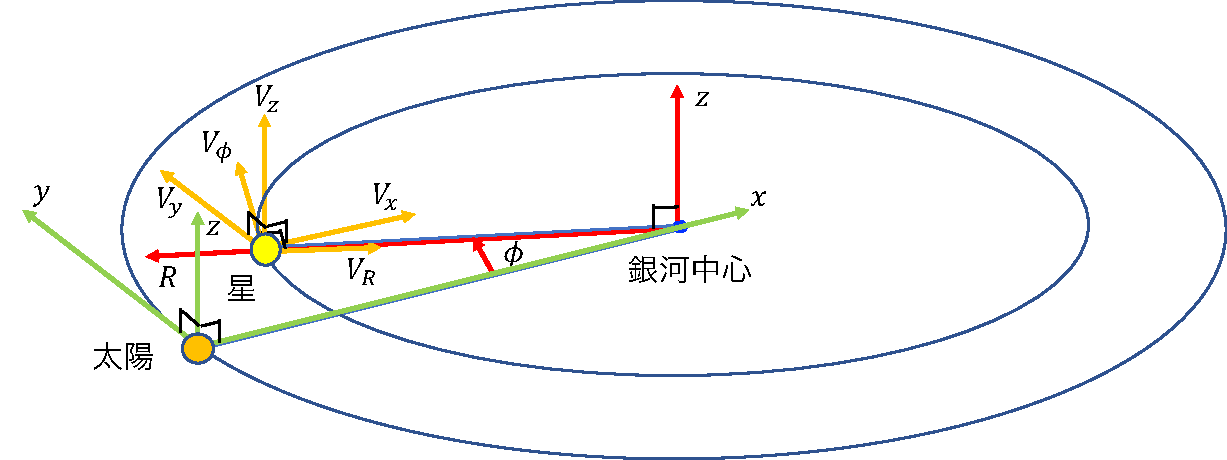
\includegraphics[width=13cm]{fig/Coordinates.pdf}
	\caption{天の川銀河を北銀極方向から斜めに下ろした図。オレンジ色の線はベクトル、緑線は太陽系を中心とした直交座標系、赤線は銀河系中心を中心とした円筒座標系、黄線は直交座標系での星の速度ベクトルを表している。}
	\label{fig:coordinates}
\end{figure*}

さらに軸対称な系では、$C=K=0$となり、
%\footnote[1]{しかしながら、$C$と$K$がゼロであることは銀河系ポテンシャルが軸対称になる上で必要ではないことに注意しなければならない。代わりに太陽が楕円ポテンシャルの主軸の近くに位置する可能性がある。(\cite{KT1994})}
\begin{subequations}
\begin{align}
	A_{\mathrm{sym}} &=\frac{1}{2}\left( \frac{v_{\phi}}{R} - \frac{\partial v_{\phi}}{\partial R} \right)_{R=R_0} \\
	B_{\mathrm{sym}} &=\frac{1}{2}\left( -\frac{v_{\phi}}{R} - \frac{\partial v_{\phi}}{\partial R} \right)_{R=R_0}
\end{align} \label{ABsym}
\end{subequations}
はオールトによって実際に得られた式である。軸対称な銀河では、閉じた軌道はほぼ円軌道と近似できるため、このときの軌道の速度$v_{\phi}$は$v_{\phi}^2=R \partial\ \Phi/\partial R$を持ち、オールト定数の測定は銀河系ポテンシャル$\Phi$の直接的な制限をすることになる。例えば、調和振動子ポテンシャル$(\Phi \propto R^2)$では、
\begin{align}
\begin{aligned}
    v_{\mathrm{c}} = R \cfrac{\partial \Phi}{\partial R} = 2R^2 \propto R^2 \to v_{\mathrm{c}} \propto R
\end{aligned}
\end{align}
から
\begin{subequations}
\begin{align}
	A &=\frac{1}{2}\left( \frac{R}{R} - \frac{\partial R}{\partial R} \right) = 0\\
	B &=\frac{1}{2}\left( -\frac{R}{R} - \frac{\partial R}{\partial R} \right) = 1
\end{align}
\end{subequations}
となる。このとき、銀河回転は剛体回転となり、$B$は銀河の回転周波数と等しくなる。また、回転曲線が平坦なとき$(v_{\phi}=\mathrm{const})$には、定数$a$を用いて$v_{\phi} = a$とすると、
\begin{subequations}
\begin{align}
	A &=\frac{1}{2}\left( \frac{a}{R} - \frac{\partial a}{\partial R} \right) = \frac{1}{2}\frac{a}{R}\\
	B &=\frac{1}{2}\left( -\frac{a}{R} - \frac{\partial a}{\partial R} \right) = -\frac{1}{2}\frac{a}{R}
\end{align}
\end{subequations}
から$A=-B$となる。さらに、全質量が銀河系中心付近に集中してケプラーポテンシャルとなっているとき$(v_{\phi} \propto R^{-1/2})$には、中心力$F$、重力定数$G$、星の質量$M$を用いると、$F = \dfrac{GM}{R^2} = \dfrac{v_{\mathrm{c}}^2}{R}$から
\begin{align}
\begin{aligned}
    v_{\mathrm{c}}^2 = \frac{GM}{R} \to v_{\mathrm{c}} \propto R^{-1/2}
\end{aligned}
\end{align}
となるため、
\begin{subequations}
\begin{align}
	A &=\frac{1}{2}\left( \frac{R^{-1/2}}{R} - \frac{\partial R^{-1/2}}{\partial R} \right) = \frac{3}{4}R^{-3/2}\\
	B &=\frac{1}{2}\left( -\frac{R^{-1/2}}{R} - \frac{\partial R^{-1/2}}{\partial R} \right) = -\frac{1}{4}R^{-3/2}
\end{align}
\end{subequations}
から$A=-3B$となる。\cite{Oort1927b}は、不定性は大きいものの、視線速度と固有運動から$A\approx 19 \mathrm{km\,s^{-1} kpc^{-1}}, B\approx -24 \mathrm{km\,s^{-1} kpc^{-1}}$という値を得た。これは、まだ天の川銀河が回転していることが定着していなかった頃のことである。このオールトの研究結果は天の川銀河が回転していることの明確な証拠となり、天の川銀河は剛体回転しているというLindbladの提案を棄却した。

銀系$l$の位置を太陽に対して速度$(U,V)$で運動している星は視線速度$v_d$、接線速度$v_l$で観測される。このとき$v_d,v_l$は
\begin{subequations}
\begin{align}
    v_d = -V_{\odot}\sin{l} - U_{\odot}\cos{l} + d(K+A\sin{2l}+C\cos{2l}) \label{eq:6} \\
    v_l = U_{\odot}\sin{l} - V_{\odot}\cos{l} + d(B-C\sin{2l}+A\cos{2l}) \label{eq:7}
\end{align}
\end{subequations}
と表される。


%%%%%%%%%%%%%%%%%%%%%%%%%%%%%%%%%%%%%%%%%%%%%%%%%%%%%%%%%%%%%%%%%%%%%%%%
%%%%%%%%%%%%%%%%%%%%%%%%%%%%%%%%%%%%%%%%%%%%%%%%%%%%%%%%%%%%%%%%%%%%%%%%
%%%%%%%%%%%%%%%%%%%%%%%%%%%%%%%%%%%%%%%%%%%%%%%%%%%%%%%%%%%%%%%%%%%%%%%%

\section{観測方程式}
実際には天の川銀河は円盤面上に全ての星が存在するような2次元の構造ではなく、星が円盤面から離れたところにも存在する3次元であるため、$v_d,v_l$の式を直接的には使えない。したがって、銀河円盤面の外の星を一般化するために以下の式を使う。
\begin{subequations}
\begin{align}
	\varpi &= d^{-1} \cos b \\
	v_{\mathrm{los}} &= v_d \cos b + v_z \sin b \\
	\mu^*_l &= \varpi v_l \\
	\mu_b &= \varpi(v_z \cos b - v_d \sin b)
\end{align} \label{OD03}
\end{subequations}
上式の表記については図(\ref{fig:OD03})を参照されたい。
\begin{figure*}[htbp]
	\centering
	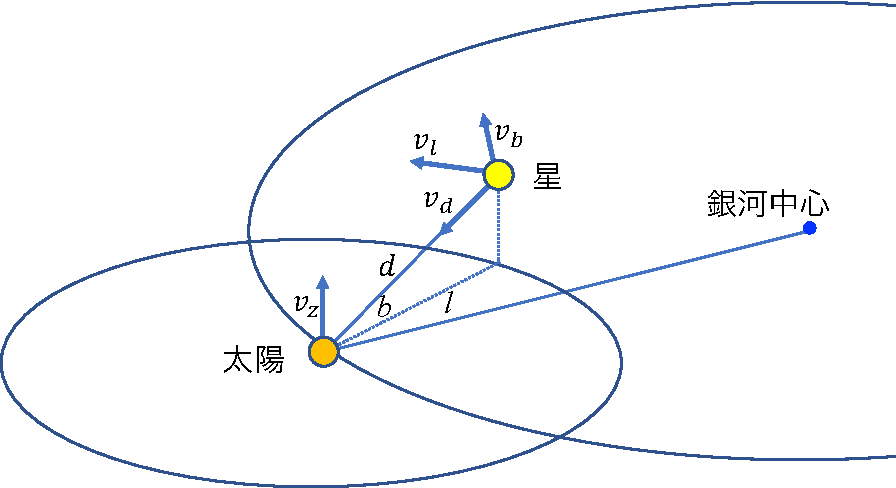
\includegraphics[width=10cm]{fig/figOD2003_2.pdf}
	\caption{式(\ref{OD03})で行っている変換で使われている各パラメータが示す量。実際の観測量は3次元の速度を持っているため、2次元モデルを使うことができるように円盤から離れた星の位置・速度を円盤面に投影する。}
	\label{fig:OD03}
\end{figure*}
このとき、
\begin{subequations}
\begin{align}
	\mu^*_l(l_i,b_i,\varpi_i) &= (A\cos2l_i - C\sin2l_i + B)\cos b_i + \varpi_i(U_{\odot}\sin l_i - V_{\odot}\cos l_i) \\
	\mu_b(l_i,b_i,\varpi_i) &= -(A\sin2l_i + C\cos2l_i + K)\sin b_i \cos b_i \nonumber \\
	                          & \hspace{2cm} + \varpi_i[(U_{\odot}\cos l_i + V_{\odot} \sin l_i)\sin b_i - W_{\odot} \cos b_i] \\
	v_{\mathrm{los}}(l_i,b_i,\varpi_i) &= (K + C\cos2l_i + A\sin2l_i)\cos^2 b_i / \varpi_i \nonumber \\
	                      & \hspace{2cm} - [(U_{\odot}\cos l_i + V_{\odot} \sin l_i)\cos b_i + W_{\odot} \sin b_i]
\end{align} \label{ObsEq}
\end{subequations}
となり、これが基本的な観測方程式となる。ここで、添字$i$は星ごとの観測量であることを示す。また$\mu^*_l \equiv \mu_l \cos b$ (観測で直接得られる値)である。

%%%%%%%%%%%%%%%%%%%%%%%%%%%%%%%%%%%%%%%%%%%%%%%%%%%%%%%%%%%%%%%%%%%%%%%%
%%%%%%%%%%%%%%%%%%%%%%%%%%%%%%%%%%%%%%%%%%%%%%%%%%%%%%%%%%%%%%%%%%%%%%%%
%%%%%%%%%%%%%%%%%%%%%%%%%%%%%%%%%%%%%%%%%%%%%%%%%%%%%%%%%%%%%%%%%%%%%%%%

\section{速度分散を考慮した場合への拡張} % Olling & Dehnenを参考に書く
前節では力学的に冷たい系、すなわち速度分散が小さく無視できる系を仮定したが、実際の銀河系円盤の星は無視できない程度の速度分散を持っている。本節では、従来のOort-Lindbladモデルによる観測方程式を速度分散を考慮した場合へ拡張することを考える。

\subsection{従来のOort-Lindbladモデルの問題点} % ここにYu & Liu の年齢速度分散関係の図も載せるとよい。
従来のOort-Lindbladモデルは速度分散が非常に小さく、ストリーミング速度に比べて無視できるような系を仮定したモデルである。しかし、現実の銀河円盤星は無視できない大きさの速度分散を持っていることが知られており、従来のモデルをそのまま用いると測定がうまくいかない可能性がある。

図\cite{YL18}によって調べられた年齢-速度分散関係である。彼らはLAMOST (Large Sky Area Multi-Object Fiber Spectroscopic Telescope) とTycho-Gaia Astrometric Solution (TGAS; \cite{Gaia2016}) をクロスマッチさせて、3564個の準巨星分枝星/赤色巨星分枝星に対して年齢推定を行った。金属量が少ない$([\mathrm{Fe}/\mathrm{H}] < 0.2\ \mathrm{dex})$星、金属量が多い$([\mathrm{Fe}/\mathrm{H}] < 0.2\ \mathrm{dex})$星と全金属量の星に関してそれぞれ年齢-速度分散関係を求めている。図\ref{VDbyYL18}を見ると、年齢と速度分散との間に明確な依存性が見られる。

\begin{figure*}[htbp]
	\centering
	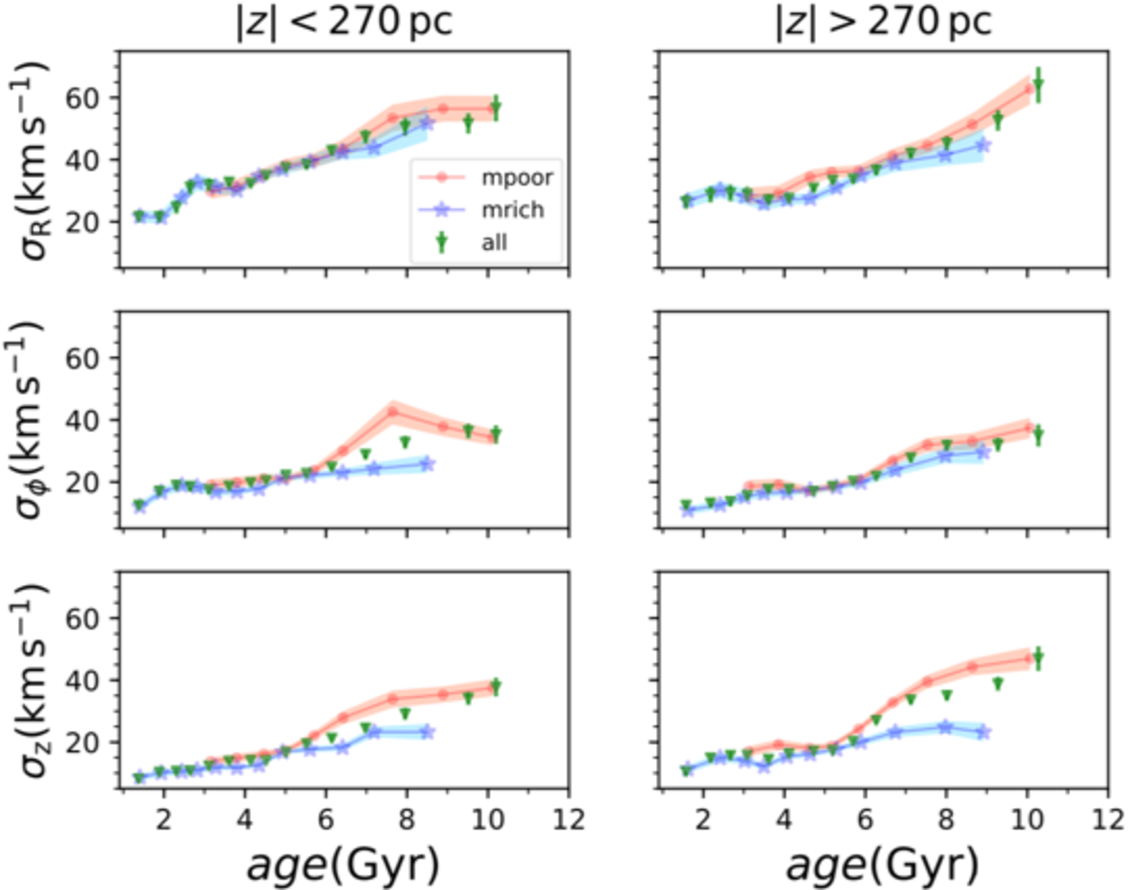
\includegraphics[width=12cm]{fig/YuLiu18_VD.pdf}
	\caption{太陽近傍星の年齢・速度分散関係\cite{YL18}。$\sigma_R,\sigma_{\phi},\sigma_z$は円筒座標系$(R,\phi,z)$での速度分散。円盤面からの距離$|z|<270\ \mathrm{pc}$と$|z|>270\ \mathrm{pc}$とで区切っている。色の違いは金属量の違いを表しており、ピンク色は金属量が少ない (metal poor) サンプル、青色は金属量が多い (metal rich) サンプル、緑色の点は両方を合わせたサンプルの速度分散となっている。}
	\label{VDbyYL18}
\end{figure*}

%%%%%%%%%%%%%%%%%%%%%%%%%%%%%%%%%%%%%%%%%%%%%%%%%%%%%%%%%%%%%%%%%%%%%

大量な星のサンプルの固有運動と視線速度からオールト定数を決定するとき、それらの値を出すときの過程と潜在的な平均速度場に関する解釈の両方を含む様々な問題に直面する。まず、若い星では運動集団や渦状腕のような非平衡な効果が平均速度$\overline{\pmb{b}}$に影響する。表\ref{table1}では、\cite{OD03}を参考にオールト定数を決定するときの問題点を挙げている。
\begin{table}[htb]
\centering
{\small
  \begin{tabular}{c|c|p{10cm}} \hline
    状態 & 表記法 & 定義と説明\\ \hline
    1 & $A,B,C,K$ & オールト定数:銀河ポテンシャル中の閉じた軌道で作られる(仮定の)速度場$\pmb{v}(\pmb{r})$の発散、回転、剪断\\
    2$^a$ & $\overline{A},\overline{B},\overline{C},\overline{K}$ & 最も得たい値:星の集団の速度場$\pmb{v}(\pmb{r})$の発散、回転、剪断\\
    3$^b$ & $\widetilde{A},\widetilde{B},\widetilde{C},\widetilde{K}$ & 実際に得られる値:星の集団から測定される固有運動のフーリエ係数\\
    \hline
  \end{tabular} \label{table1}
\vskip 3pt
\begin{minipage}{13cm}
\textit{$^a$}状態1と2の違いの理由として考えられるものを挙げる。(i)若い星:運動集団や渦状腕のような非平衡の効果が閉じた軌道の速度場から$\pmb{\overline{v}}$を予想外な値に導く。これは主に小さい速度分散の集団に影響する。(ii)サンプルの大きさが小さすぎる場合、ストリーミング場(streaming field)の中の太陽近傍の変則的なものがオールト定数に反映される。 \\
\textit{$^b$}状態2と3の違いの理由として考えられるものを挙げる。
\end{minipage}
}
\end{table}

\subsubsection{力学的に冷たい極限からのずれ}
すでに\cite{Oort1928}やその後\cite{KT1994}で指摘されているように、力学的に冷たい極限でのみランダム運動は消え私たちは平均ストリーミング速度$\overline{v}$を銀河系ポテンシャルで支えられる閉じた軌道の速度$v$として扱うことができる。一般には、そこには系統的な違いがあり、次のように書ける。
\begin{align}
\begin{aligned}
    \overline{\pmb{v}} = \pmb{v} - \pmb{v}_{\mathrm{a}}
\end{aligned} \label{AD}
\end{align}
ここで、$v_{\mathrm{a}}$はasymmetric drift速度である。asymmetric driftについての詳細は\ref{Asymmetric drift}で述べる。 driftは近傍の閉じた軌道の平均速度からの遅れを表す。この区別を明確にするために、式(\ref{AD})のようにオールト定数を書く。
\begin{subequations}
\begin{align}
	\overline{A} &= A - A_{\mathrm{a}} \\
	\overline{B} &= B - B_{\mathrm{a}} \\
	\overline{C} &= C - C_{\mathrm{a}} \\
	\overline{K} &= K - K_{\mathrm{a}}
\end{align}
\end{subequations}
(仮定の)閉じた軌道のストリーミング場から$A,B,C,K$出され、ポテンシャルに従った項で直接的に解釈される一方、$\overline{A},\overline{B},\overline{C},\overline{K}$は実際の星の集団のストリーミング場を表す。$\overline{A},\overline{B},\overline{C},\overline{K}$は式(\ref{eq2})あるいは(\ref{eq2.5a})-(\ref{eq2.5d})において$\pmb{v}$を$\pmb{\overline{v}}$で置き換えたもので、$A_{\mathrm{a}},B_{\mathrm{a}},C_{\mathrm{a}},K_{\mathrm{a}}$は同じく$\pmb{v}$を$\pmb{v}_{\mathrm{a}}$で置き換えたものである。近傍のストリーミング速度との相対的な太陽運動はLSR(Local Standard of Rest)に対しての太陽運動とasymmetric driftとに分解される(図\ref{fig1})。

\begin{figure*}[htbp]
	\centering
	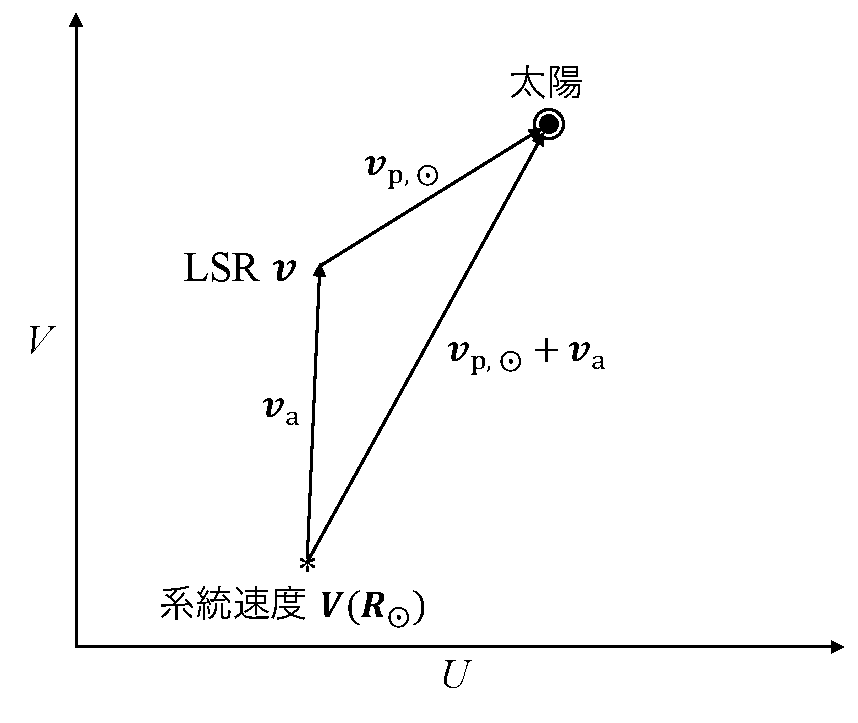
\includegraphics[width=10cm]{fig/various_velocities.pdf}
	\caption{太陽運動とasymmetric driftのスケッチ。サンプル星の平均ストリーミング速度$\pmb{\overline{v}}$は速度$\pmb{v}$LSRからasymmetric drift$\pmb{v}_{\mathrm{a}}$の分遅れる。太陽の特異運動$\pmb{v}_{\odot}$は観測されたストリーミング速度$\pmb{\overline{v}}$に対する太陽の速度を得るために$\pmb{v}_{\mathrm{a}}$を足す必要がある。}
	\label{fig1}
\end{figure*}

軸対称な銀河では、方位角成分$v_{\mathrm{a}}$のみが存在し、ランダム運動は回転速度に比べて非常に小さく、これはStr\"{o}mbergの関係(Jeans方程式からの導出は\cite{BT2008}、\ref{Asymmetric drift}章を参照)から近似される。
\begin{align}
\begin{aligned}
    v_{\mathrm{a}} \simeq \frac{\overline{v_{\mathrm{los}}^2}}{2v_{\phi}} \left[\frac{\sigma_{\phi}^2}{\overline{v_{\mathrm{los}}^2}} - 1 - \frac{\partial \ln(\nu \overline{v_{\mathrm{los}}^2})}{\partial \ln R} - \frac{R}{\overline{v_{\mathrm{los}}^2}}\frac{\partial \overline{v_{\mathrm{los}} v_z}}{\partial z}\right] \\
    = \frac{\sigma_R^2}{2v_{\phi}} \left[\frac{\sigma_{\phi}^2}{\sigma_R^2} - 1 - \frac{\partial \ln(\nu \sigma_R^2)}{\partial \ln R} - \frac{R}{\sigma_R^2}\frac{\partial \sigma_{Rz}^2}{\partial z}\right]
\end{aligned} \label{AD2}
\end{align}
ここで、$\nu$は星密度、$\sigma_{ij}^2 \equiv \overline{(v_i-\overline{v_i})(v_j-\overline{v_j})}=\overline{v_i v_j}-\overline{v_i}\ \overline{v_j}$は速度分散テンソルを示し、ここでは広く使われるように$\sigma_{ii}^2$を$\sigma_i^2$と短く書いている。式(\ref{AD2})の1行目から2行目への式変形では$\overline{v_{\mathrm{los}}}=0$と仮定している。従って、asymmetric driftは動径速度分散の関数であり、円軌道速度と速度楕円体の軸比、動径速度分散と星密度の傾きにも依存する。この関係を予測されるオールト定数$A,B$への影響を推定することに使うことができる。視線方向と接線方向の速度分散の動径方向への依存性の決定については\cite{LF1989}を参照されたい。式(\ref{AD2})の最後の項の動径方向の変化を無視し、$\nu,\sigma_{ij}^2$がそれぞれスケール長$R_d,R_{\sigma^2}$で指数関数的に変化すると仮定すると、
\begin{align}
\begin{aligned}
    \frac{\partial \ln v_{\mathrm{a}}}{\partial R} \simeq -\frac{1}{R_{\sigma^2}} + \frac{k}{2v_{\phi}}\left(\frac{1}{R_d} + \frac{1}{R_{\sigma^2}}\right) - \frac{\partial \ln v_{\phi}}{\partial R}
\end{aligned} \label{AD3}
\end{align}
と書ける。ここで、$kv_{\mathrm{a}} \simeq \sigma_{R}^2, k=80 \pm 5 \mathrm{km\ s^{-1}}$(\cite{DB1998})という関係を用いた。

式(\ref{AD2})から式(\ref{AD3})への変形について
\begin{align}
\begin{aligned}
    v_{\mathrm{a}} \simeq \frac{\sigma_R^2}{2v_{\phi}} \left[\frac{\sigma_{\phi}^2}{\sigma_R^2} - 1 - \frac{\partial \mathrm{ln}(\nu \sigma_R^2)}{\partial \mathrm{ln} R} - \frac{R}{\sigma_R^2}\frac{\partial \sigma_{Rz}^2}{\partial z}\right]
\end{aligned} \label{AD4}
\end{align}
ここで、$\nu \propto e^{
-R/R_d},\sigma_{ij}^2 \propto e^{-R/R_{\sigma}^2}, kv_{\mathrm{a}} \simeq \sigma_{R}^2$という仮定を用いる。まず、式(\ref{AD4})の右辺第3項は$-\partial \mathrm{ln}(\nu \sigma_R^2)/\partial \mathrm{ln} R = R(1/R_d + 1/R_{\sigma^2})$と変形できる。さらに第4項は無視できるから、
\begin{align}
\begin{aligned}
    2v_{\phi}v_{\mathrm{a}} \simeq \sigma_R^2 \left[\frac{\sigma_{\phi}^2}{\sigma_R^2} - 1 + R\left(\frac{1}{R_d} + \frac{1}{R_{\sigma^2}}\right)\right]
\end{aligned} \label{AD5}
\end{align}
となる。ここで、$\sigma_{ij}^2 \propto e^{-R/R_{\sigma^2}}$から、$D$を定数として$\sigma_{\phi}^2/\sigma_R^2 - 1 = D$と書けるから、
\begin{align}
\begin{aligned}
    2v_{\phi}v_{\mathrm{a}} \simeq \sigma_R^2 \left[D + R\left(\frac{1}{R_d} + \frac{1}{R_{\sigma^2}}\right)\right]
\end{aligned} \label{AD6}
\end{align}
式 (\ref{AD6})の両辺のlogをとり$R$で微分すると、
\begin{align}
\begin{aligned}
    \ln2+\ln v_{\phi}+\ln v_{\mathrm{a}} &\simeq \ln \sigma_R^2 +\ln \left[D + R\left(\frac{1}{R_d} + \frac{1}{R_{\sigma^2}}\right)\right] \\
    \frac{\partial \ln v_{\phi}}{\partial R}+\frac{\partial \ln v_{\mathrm{a}}}{\partial R} &\simeq -\frac{1}{R_{\sigma^2}} + \frac{1/R_d + 1/R_{\sigma^2}}{D +R\left(1/R_d + 1/R_{\sigma^2}\right)} \\
\end{aligned} \label{AD8}
\end{align}
したがって、式(\ref{AD6}),(\ref{AD8})と$kv_{\mathrm{a}} \simeq \sigma_R^2$から
\begin{align}
\begin{aligned}
    \frac{\partial \mathrm{ln}v_{\mathrm{a}}}{\partial R} \simeq -\frac{1}{R_{\sigma^2}} + \frac{k}{2v_{\phi}}\left(\frac{1}{R_d} + \frac{1}{R_{\sigma^2}}\right) - \frac{\partial \mathrm{ln}v_{\phi}}{\partial R}
\end{aligned} \label{AD9}
\end{align}
となる。

asymmetric driftは軸対称を仮定していることから、式(\ref{ABsym})を利用して$A_{\mathrm{a}},B_{\mathrm{a}}$は次のように表すことができる。
\begin{subequations}
\begin{align}
	A_{\mathrm{a}} &=\frac{1}{2}\left( \frac{v_{\mathrm{a}}}{R} - \frac{\partial v_{\mathrm{a}}}{\partial R} \right)_{R=R_0} \\
	B_{\mathrm{a}} &=\frac{1}{2}\left( -\frac{v_{\mathrm{a}}}{R} - \frac{\partial v_{\mathrm{a}}}{\partial R} \right)_{R=R_0}
\end{align} \label{ABaxisym}
\end{subequations}
さらに式(\ref{AD3})を利用すると、$R_{\sigma^2}=0.45R_0$(\cite{LF1989})とするとき$A_{\mathrm{a}}\approx0.14v_{\mathrm{a}}, B_{\mathrm{a}}\approx0.04v_{\mathrm{a}}$となり、$R_d,R_0,v_{\phi}$とはほぼ独立している。すなわち、$B$はasymmetric driftの影響をほとんど受けないが、$A_{\mathrm{a}}$は$v_{\mathrm{a}}=20$のときには3程度の大きさとなり、asymmetric driftの影響を少し受ける。

%%%%%%%%%%%%%%%%%%%%%%%%%%%%%%%%%%%%%%%%%%%%%%%%%%%%%%%%%%
%%%%%%%%%%%%%%%%%%%%%%%%%%%%%%%%%%%%%%%%%%%%%%%%%%%%%%%%%%
%%%%%%%%%%%%%%%%%%%%%%%%%%%%%%%%%%%%%%%%%%%%%%%%%%%%%%%%%%


\subsection{asymmetric drift} % 導出&物理的解釈を書く
\subsection{asymmetric driftを考慮した観測方程式}
ここで、観測方程式にasymmetric drift項を追加することを考える。円筒座標系で$(0,v_a,0)$とする。銀河座標系でのasymmetric drift項を$(v_{a,l},v_{a,b},v_{a,\gamma})$と書くと、
\begin{align}
\begin{aligned}
	\left(
	\begin{array}{c}
	 	v_{a,l}\\
		v_{a,b}\\
		v_{a,\gamma}
	\end{array}
	\right)
	=& \bf{P} \bf{Q}
	\left(
	\begin{array}{c}
	 	0\\
		v_a\\
		0
	\end{array}
	\right)
\end{aligned}
\end{align}
となる。ここで、$\bf{P,Q}$はそれぞれ$(v_{\mathrm{los}},v_{\phi},v_z) \to (v_x,v_ y,v_z), (v_x,v_y,v_z) \to (v_l,v_ b,v_{\mathrm{los}})$のようにベクトルを変換する行列である。式(\ref{ObsEq})にasymmetric drift項を追加した式は
\begin{subequations}
\begin{align}
	\mu^*_l(l_i,b_i,\varpi_i) &= (A\cos2l_i - C\sin2l_i + B)\cos b_i + \varpi_i(U_{\odot}\sin l_i - V_{\odot}\cos l_i) - \varpi_i v_{a,l} \\
	\mu_b(l_i,b_i,\varpi_i) &= -(A\sin2l_i + C\cos2l_i + K)\sin b_i \cos b_i \nonumber \\
	                          & \hspace{2cm} + \varpi_i[(U_{\odot}\cos l_i + V_{\odot} \sin l_i)\sin b_i - W_{\odot} \cos b_i] - \varpi_i v_{a,b} \\
	v_{\mathrm{los}}(l_i,b_i,\varpi_i) &= (K + C\cos2l_i + A\sin2l_i)\cos^2 b_i / \varpi \nonumber \\
	                      & \hspace{2cm} - [(U_{\odot}\cos l_i + V_{\odot} \sin l_i)\cos b_i + W_{\odot} \sin b_i] - v_{a,\gamma}
\end{align} \label{ObsEqAD}
\end{subequations}
となる。



%%%%%%%%%%%%%%%%%%%%%%%%%%%%%%%%%%%%%%%%%%%%%%%%%%%%%%%%%%%%%%%%%%%%%%%%
%%%%%%%%%%%%%%%%%%%%%%%%%%%%%%%%%%%%%%%%%%%%%%%%%%%%%%%%%%%%%%%%%%%%%%%%
%%%%%%%%%%%%%%%%%%%%%%%%%%%%%%%%%%%%%%%%%%%%%%%%%%%%%%%%%%%%%%%%%%%%%%%%
% ここからコメントアウト

\begin{comment}




%%%%%%%%%%%%%%%%%%%%%%%%%%%%%%%%%%%%%%%%%%%%%%%%%%%%%%%%%%%%%%%%%%%%%%%%%%%%%%%%%%%%%%%%%%%%%%%%
%%%%%%%%%%%%%%%%%%%%%%%%%%%%%%%%%%%%%%%%%%%%%%%%%%%%%%%%%%%%%%%%%%%%%%%%%%%%%%%%%%%%%%%%%%%%%%%%
%%%%%%%%%%%%%%%%%%%%%%%%%%%%%%%%%%%%%%%%%%%%%%%%%%%%%%%%%%%%%%%%%%%%%%%%%%%%%%%%%%%%%%%%%%%%%%%%


\section{Asymmetric drift \label{Asymmetric drift}}
この節では\cite{BT08}にしたがってasymmetric driftについて説明する。

重力ポテンシャルが$\Phi$のとき$H=\frac{1}{2}v^2 + \Phi(\pmb{x},t)$で書けるような直交座標系での無衝突ボルツマン方程式は次のようになる。
\begin{align}
	\frac{\partial f}{\partial t} + p_R\frac{\partial f}{\partial R} + \frac{p_{\phi}}{R^2}\frac{\partial f}{\partial \phi} + p_z\frac{\partial f}{\partial z} - \left(\frac{\partial \Phi}{\partial R} - \frac{p_{\phi}^2}{R^3} \right)\frac{\partial f}{\partial p_R} - \frac{\partial \Phi}{\partial \phi}\frac{\partial f}{\partial p_{\phi}} - \frac{\partial \Phi}{\partial z}\frac{\partial f}{\partial p_z} = 0
\end{align}
円筒座標系では$H = \frac{1}{2}(p_R^2 + p_{\phi}^2/R^2 + p_z^2) + \Phi$となり、そのため
\begin{align}
	\frac{\partial f}{\partial t} + \frac{\partial f}{\partial \pmb{q}} \frac{\partial H}{\partial \pmb{p}} - \frac{\partial f}{\partial \pmb{p}} \frac{\partial H}{\partial \pmb{q}} = 0
\end{align}
から
\begin{align}
	\frac{\partial f}{\partial t} + p_R\frac{\partial f}{\partial R} + \frac{p_{\phi}}{R^2}\frac{\partial f}{\partial \phi} + p_z\frac{\partial f}{\partial z} - \left(\frac{\partial \Phi}{\partial R} - \frac{p_{\phi}^2}{R^3} \right)\frac{\partial f}{\partial p_R} - \frac{\partial \Phi}{\partial \phi}\frac{\partial f}{\partial p_{\phi}} - \frac{\partial \Phi}{\partial z}\frac{\partial f}{\partial p_z} = 0   \label{eq193}
\end{align}
のようになる。考えている系が定常状態で軸対称であると仮定すると、$t$と$\phi$に関する微分の項は全て消える。これらの仮定から、式(\ref{eq193})は
\begin{align}
	p_r\frac{\partial f}{\partial R} + p_z\frac{\partial f}{\partial z} - \left(\frac{\partial \Phi}{\partial R} - \frac{p_{\phi}^2}{R^3} \right)\frac{\partial f}{\partial p_R} - \frac{\partial \Phi}{\partial z}\frac{\partial f}{\partial p_z} = 0    \label{eq196}
\end{align}
と簡単に書ける。この式に$p_R$をかけて全運動量で積分し、式(\ref{eq196})を用いて
\begin{align}
	\frac{\partial (\nu \overline{v_{\mathrm{los}}^2})}{\partial R} + \frac{\partial (\nu \overline{v_{\mathrm{los}} v_z})}{\partial R} + \nu\left(\frac{\overline{v_{\mathrm{los}}^2} - \overline{v_{\phi}^2}}{R} + \frac{\partial \Phi}{\partial R} \right) = 0   \label{eq200}
\end{align}
となる。ここで、asymmetric drift速度
\begin{align}
	v_{\mathrm a} \equiv v_{\mathrm c} - \overline{v_{\phi}}
\end{align}
を考える。$v_{\mathrm c}$は太陽近傍での円軌道速度である。

今、円盤は定常状態でその赤道面に対して対称であると考える。また、太陽は銀河赤道の近くに位置しているため、$z=0$での式(\ref{eq200})を考えればよい。対称性より$\partial \nu/\partial z = 0$であるから、次の式を得る。
\begin{align}
	\frac{R}{\nu}\frac{\partial(\nu \overline{v_{\mathrm{los}}^2})}{\partial R} + R\frac{\partial(\overline{v_{\mathrm{los}} v_z})}{\partial z} + \overline{v_{\mathrm{los}}^2} - \overline{v_{\phi}^2} + R\frac{\partial \Phi}{\partial R} = 0
\end{align}
$\sigma_{ij}^2 = \overline{v_i v_j} - \overline{v_i}\overline{v_j}$とasymmetric driftの定義から、
\begin{align}
	\sigma_{\phi}^2 - \overline{v_{\mathrm{los}}^2} &-\frac{R}{\nu}\frac{\partial(\nu \overline{v_{\mathrm{los}}^2})}{\partial R} - R\frac{\partial(\overline{v_{\mathrm{los}} v_z})}{\partial z} = v_{\mathrm c}^2 - \overline{v_{\phi}^2} \\
	&= (v_{\mathrm c} - \overline{v_{\phi}}) (v_{\mathrm c} + \overline{v_{\phi}}) = v_{\mathrm a}(2v_{\mathrm c} - v_{\mathrm a})
\end{align}
となる。$2v_{\mathrm c}$に比べて$v_{\mathrm a}$が無視できるとき、Str\"{o}mbergのasymmetric drift方程式
\begin{align}
	v_{\mathrm a} \simeq \frac{\overline{v_{\mathrm{los}}^2}}{2v_{\mathrm c}}\left[\frac{\sigma_{\phi}^2}{\overline{v_{\mathrm{los}}^2}} - 1 - \frac{\partial\ln(\nu\overline{v_{\mathrm{los}}^2})}{\partial\ln R} - \frac{R}{\overline{v_{\mathrm{los}}^2}}\frac{\partial(\overline{v_{\mathrm{los}} v_z})}{\partial z}\right]   \label{eq221}
\end{align}
が得られる。

\cite{BM1998}の表10.2から、$\sigma_{\phi}^2/\overline{v_{\mathrm{los}}^2}=0.35$という値を使用することにする。$\nu,\overline{v_{\mathrm{los}}^2}$はともに$e^{-R/R_{\mathrm d}}$に比例し、$R/R_{\mathrm d}=3.2$と仮定する。以上の仮定を用いると、式(\ref{eq221})の角括弧内の前の3項の合計は5.8となる。最後の項は銀河系円盤面のちょうど上の点での速度楕円体の向きに依存するため、測定することが難しい。これについては次の2つの極限での可能性がある。座標系の中心は銀河中心とし、(1)楕円体の主軸が円筒座標系$(R,\phi,z)$の座標軸に沿った向き、(2)主軸が球対称座標系$(R,\theta,\phi)$の座標軸に沿った向きになる場合に2つの可能性である。軌道積分(\cite{BS1983})は、実際にはこの2つの可能性のほぼ真ん中の状態になっていると示唆している。(1)の場合では$\overline{v_{\mathrm{los}} v_z}$はzに関して独立であり、(2)に場合では$\overline{v_{\mathrm{los}} v_z}\simeq (\overline{v_{\mathrm{los}}^2}-\overline{v_z^2})(z/R)$と書け、この項は$-(1-\overline{v_z^2}/\overline{v_{\mathrm{los}}^2})\simeq -0.8$となる。これらの値の平均をとると、角括弧内の値は$5.4\pm 0.4$となり、そのため$v_{\mathrm a}\simeq \overline{v_{\mathrm{los}}^2}/(81.5 \pm 6 \ \mathrm{km\ s^{-1}})$となる。

本研究ではまず$\overline{v_{\mathrm{los}}}=0 \mathrm{km\ s^{-1}}$と仮定し、$\sigma_{v_{\mathrm{los}}}^2 = \overline{v_{\mathrm{los}}^2}$とする。さらに、$\nu \propto e^{-R/h_R}, \sigma_{vR} \propto e^{-R/h_{\sigma}}$と仮定する。ここで、$h_R,h_{\sigma}$はそれぞれ星の密度分布のスケール長、速度分散のスケール長である。\cite{Bovy2012b}では$h_R=3 \mathrm{kpc},h_{\sigma}=8 \mathrm{kpc}$、\cite{Kawata2019}では$h_R=20 \mathrm{kpc},h_{\sigma}=20 \mathrm{kpc}$が使用されていたが、\cite{BH2016}の表5から本研究では$h_R=2.5 \mathrm{kpc},h_{\sigma}=8 \mathrm{kpc}$を採用する。また、式(\ref{eq221})の角括弧内の最後の項は\cite{BT08}と同様の値を採用する。これらのことから、asymmetric driftは
\begin{align}
	v_{\mathrm a} &\simeq \frac{\sigma_{R}^2}{2v_{\mathrm c}}\left[\frac{\sigma_{\phi}^2}{\sigma_{R}^2} - 1 - \frac{\partial\ln(\nu\sigma_{R}^2)}{\partial\ln R} - \frac{R}{\overline{v_{\mathrm{los}}^2}}\frac{\partial(\overline{v_{\mathrm{los}} v_z})}{\partial z}\right]\\
	&= \simeq \frac{\sigma_{R}^2}{2v_{\mathrm c}}\left[\frac{\sigma_{\phi}^2}{\sigma_{R}^2} + R\left(\frac{1}{h_R}+\frac{2}{h_{\sigma}}\right) - 1.4\right]
\end{align} \label{AD244}
となる。


%%%%%%%%%%%%%%%%%%%%%%%%%%%%%%%%%%%%%%%%%%%%%%%%%%%%%%%%%%%%%%%%%%%%%%%%%%%%%%%%%%%%%%%%%%%%%%%%
%%%%%%%%%%%%%%%%%%%%%%%%%%%%%%%%%%%%%%%%%%%%%%%%%%%%%%%%%%%%%%%%%%%%%%%%%%%%%%%%%%%%%%%%%%%%%%%%
%%%%%%%%%%%%%%%%%%%%%%%%%%%%%%%%%%%%%%%%%%%%%%%%%%%%%%%%%%%%%%%%%%%%%%%%%%%%%%%%%%%%%%%%%%%%%%%%

\section{速度楕円体}
空間上のある$i$方向の速度分散は$\sigma_i^2 \equiv \overline{(v_i-\overline{v_i})}^2$、$i$方向と$j$方向の間の速度分散テンソルは$\sigma_{ij}^2 \equiv \overline{(v_i-\overline{v_i})(v_j-\overline{v_j})}$と定義される。このとき、$\sigma_i$を半長軸とする楕円体を定義でき、これを速度楕円体と呼ぶ。速度楕円体は一般に3軸非対称であり、半長軸の方向は座標軸とは一致するとは限らない。速度楕円体の長軸と座標軸との傾き、例えば$i$軸から$j$軸に向かって$l_{ij}$だけ傾いているとき、
\begin{align}
    \tan(2l_{ij}) = \frac{2\sigma _{ij}^2}{\sigma_i^2 \sigma_j^2}
\end{align}
と表すことができる。

\begin{figure*}[htbp]
	\centering
	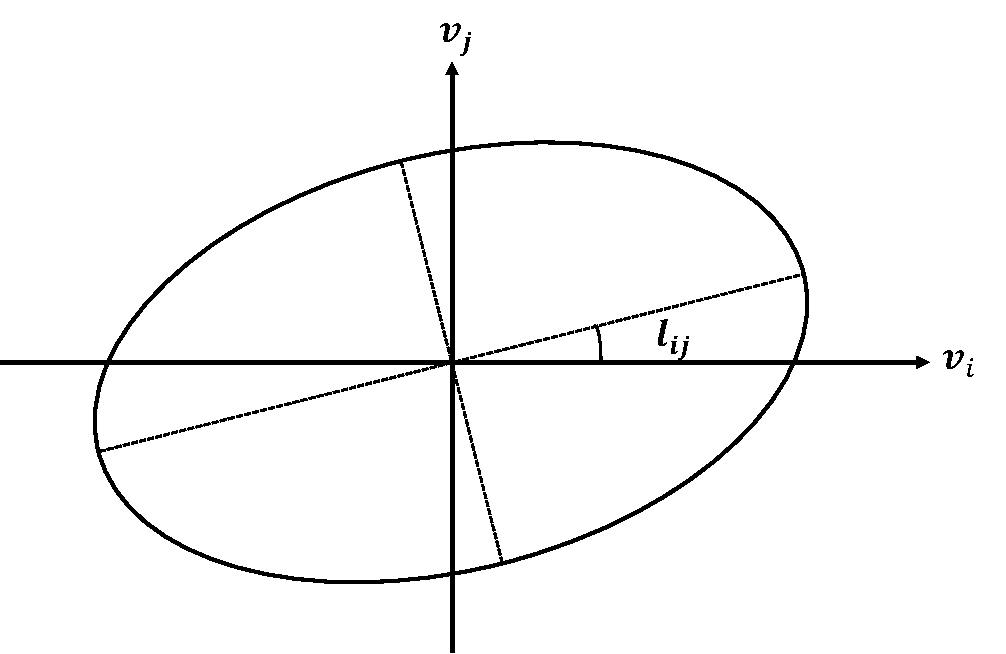
\includegraphics[width=13cm]{fig/velocity_ellipsoid.pdf}
	\caption{速度楕円体を2次元に投影したときの図。楕円は速度分散の1$\sigma$にあたる点を結んだ線である。$l_{ij}$は座標軸を図のようにとったときの楕円の主軸との傾きを表す。}
	\label{fig:ve}
\end{figure*}


\end{comment}